\section{Abstractor architectures}\label{sec:abstractor_architectures}

% Similar to a Transformer Encoder, an Abstractor is a module that takes a sequence of objects $X = (x_1, \ldots, x_\m)$ as input and produces a processed representation of the input as another sequence of objects, $A = (A_1, \ldots, A_\m)$. In contrast to the encoder states $E = \paren{E_1, \ldots, E_\m}$, which represent an entangled mixture of object-level attributes and relational information, the abstract states $A$ represent only relational information of the input, abstracted away from the object-level attributes. An Abstractor is a module whose purpose is to process purely relational information. It can be integrated into a broader transformer-based architecture in several different ways, depending on the target task.

Whereas an Encoder performs ``general-purpose'' processing, extracting representations of both object-level and relational information, an Abstractor module is more specialized and produces purely relational representations. An Abstractor can be integrated into a broader transformer-based architecture, for enhanced relational processing.

To facilitate the discussion of different architectures, we distinguish between two types of tasks. In a \textit{purely relational} prediction task, there exists a sufficient statistic of the input which is purely relational and encodes all the information that is relevant for predicting the target. The experiments of~\citep{esbn,kerg2022neural} are examples of discriminative purely relational tasks. An example of a sequence-to-sequence purely relational task is the object-sorting task described in~\Cref{ssec:experiments_object_sorting}.
% To predict the `argsort' of a sequence of objects, the pairwise $\prec$ relation is sufficient.
Many real-world tasks, however, are not purely relational. In a \textit{partially-relational} prediction task, the relational information is important, but it is not sufficient for predicting the target. Natural language understanding is an example of a partially-relational task. The math problem-solving experiments in~\Cref{ssec:experiments_math} are also partially-relational.

\begin{figure}
    \centering
    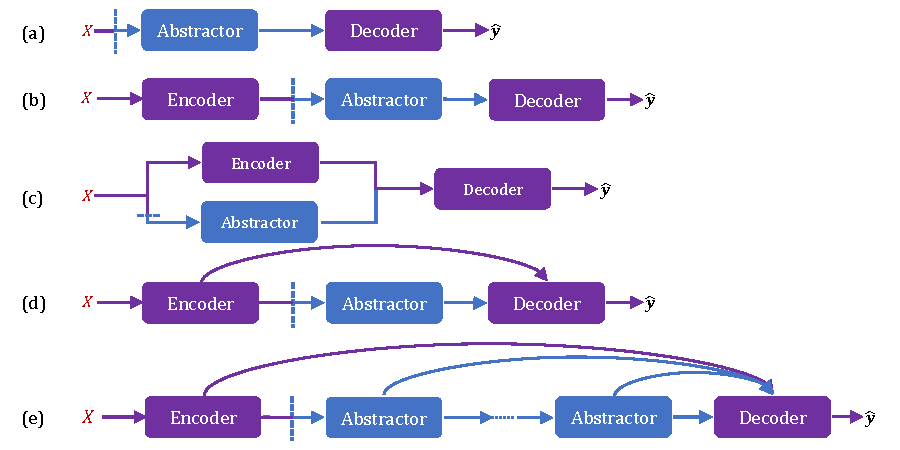
\includegraphics[width=.8\textwidth]{figures/abstractor_architectures.pdf}
    \caption{Examples of Abstractor-based model architectures.}\label{fig:abstractor_architectures}
    \vskip-10pt
\end{figure}


The way that an Abstractor module is integrated into a broader model architecture should be informed by the underlying prediction task.~\Cref{fig:abstractor_architectures} depicts several Abstractor architectures each with different properties. Architecture (a) depicts an architecture in which the Abstractor processes the relational features in the input, and the decoder attends to the abstract states $A$. Architecture (b) depicts a model in which the input objects are first processed by an Encoder, followed by an Abstractor for relational processing, and the decoder again attends to the abstract states. These architectures would be appropriate for purely relational tasks since the decoder attends only to the relational representations in the abstract states. Architectures (c) and (d) would be more appropriate for more general tasks which are only partially relational. For example, in architecture (c), the model branches into two parallel processing streams in which an Encoder performs general-purpose processing and an Abstractor performs more specialized processing of relational information.
The decoder attends to \textit{both} the encoder states and abstract states.
% We refer to architectures which combine sensory processing with abstract relational processing as \textit{sensory-connected} architectures.
These architectures use the ``multi-attention decoder'' described in~\Cref{sec:multi_attn_decoder}.
Finally, architecture (e) depicts a \textit{composition} of Abstractors, wherein the abstract states produced by one Abstractor module are used as input to another Abstractor. This results in computing ``higher-order'' relational information (i.e., relations on relations).
% This is made formal in~\Cref{ssec:function_classes_preview}. % we cut out the abstractor theory section. hopefully we can include it in a final version?
% We leave empirical evaluation of this architecture to future work. 